%%%%%%%%%%%%%%%%%%%%%%%%%%%%%%%%%%%%%%%%%%%%%%%%%%%%%%%%%%%%%%%%%%%%%%%%%%%%%%%

\section*{\large Exercício 9 - Self-Organized Criticality (SOC)}
\addcontentsline{toc}{chapter}{\protect\numberline{}\large Exercício 9}%

Os resultados deste exercício se encontram na pasta \textbf{Exercise9}, organizados nas pastas \textbf{9.1} e \textbf{9.2}.

\subsection*{9.1}
\addcontentsline{toc}{section}{\protect\numberline{} 9.1}%

O resultado a seguir resume a aplicação do algoritmo SOC.py às séries endógenas e exógenas do p-model. Pode-se observar que as séries endógenas apresentam Self Organized Criticality.

\begin{figure}[ht!]
	%\caption{Série e histogramas.}
	\vspace{0mm}	% acrescentar o espaçamento vertical apropriado entre o título e a borda superior da figura
	\begin{center}
		\resizebox{15cm}{!}{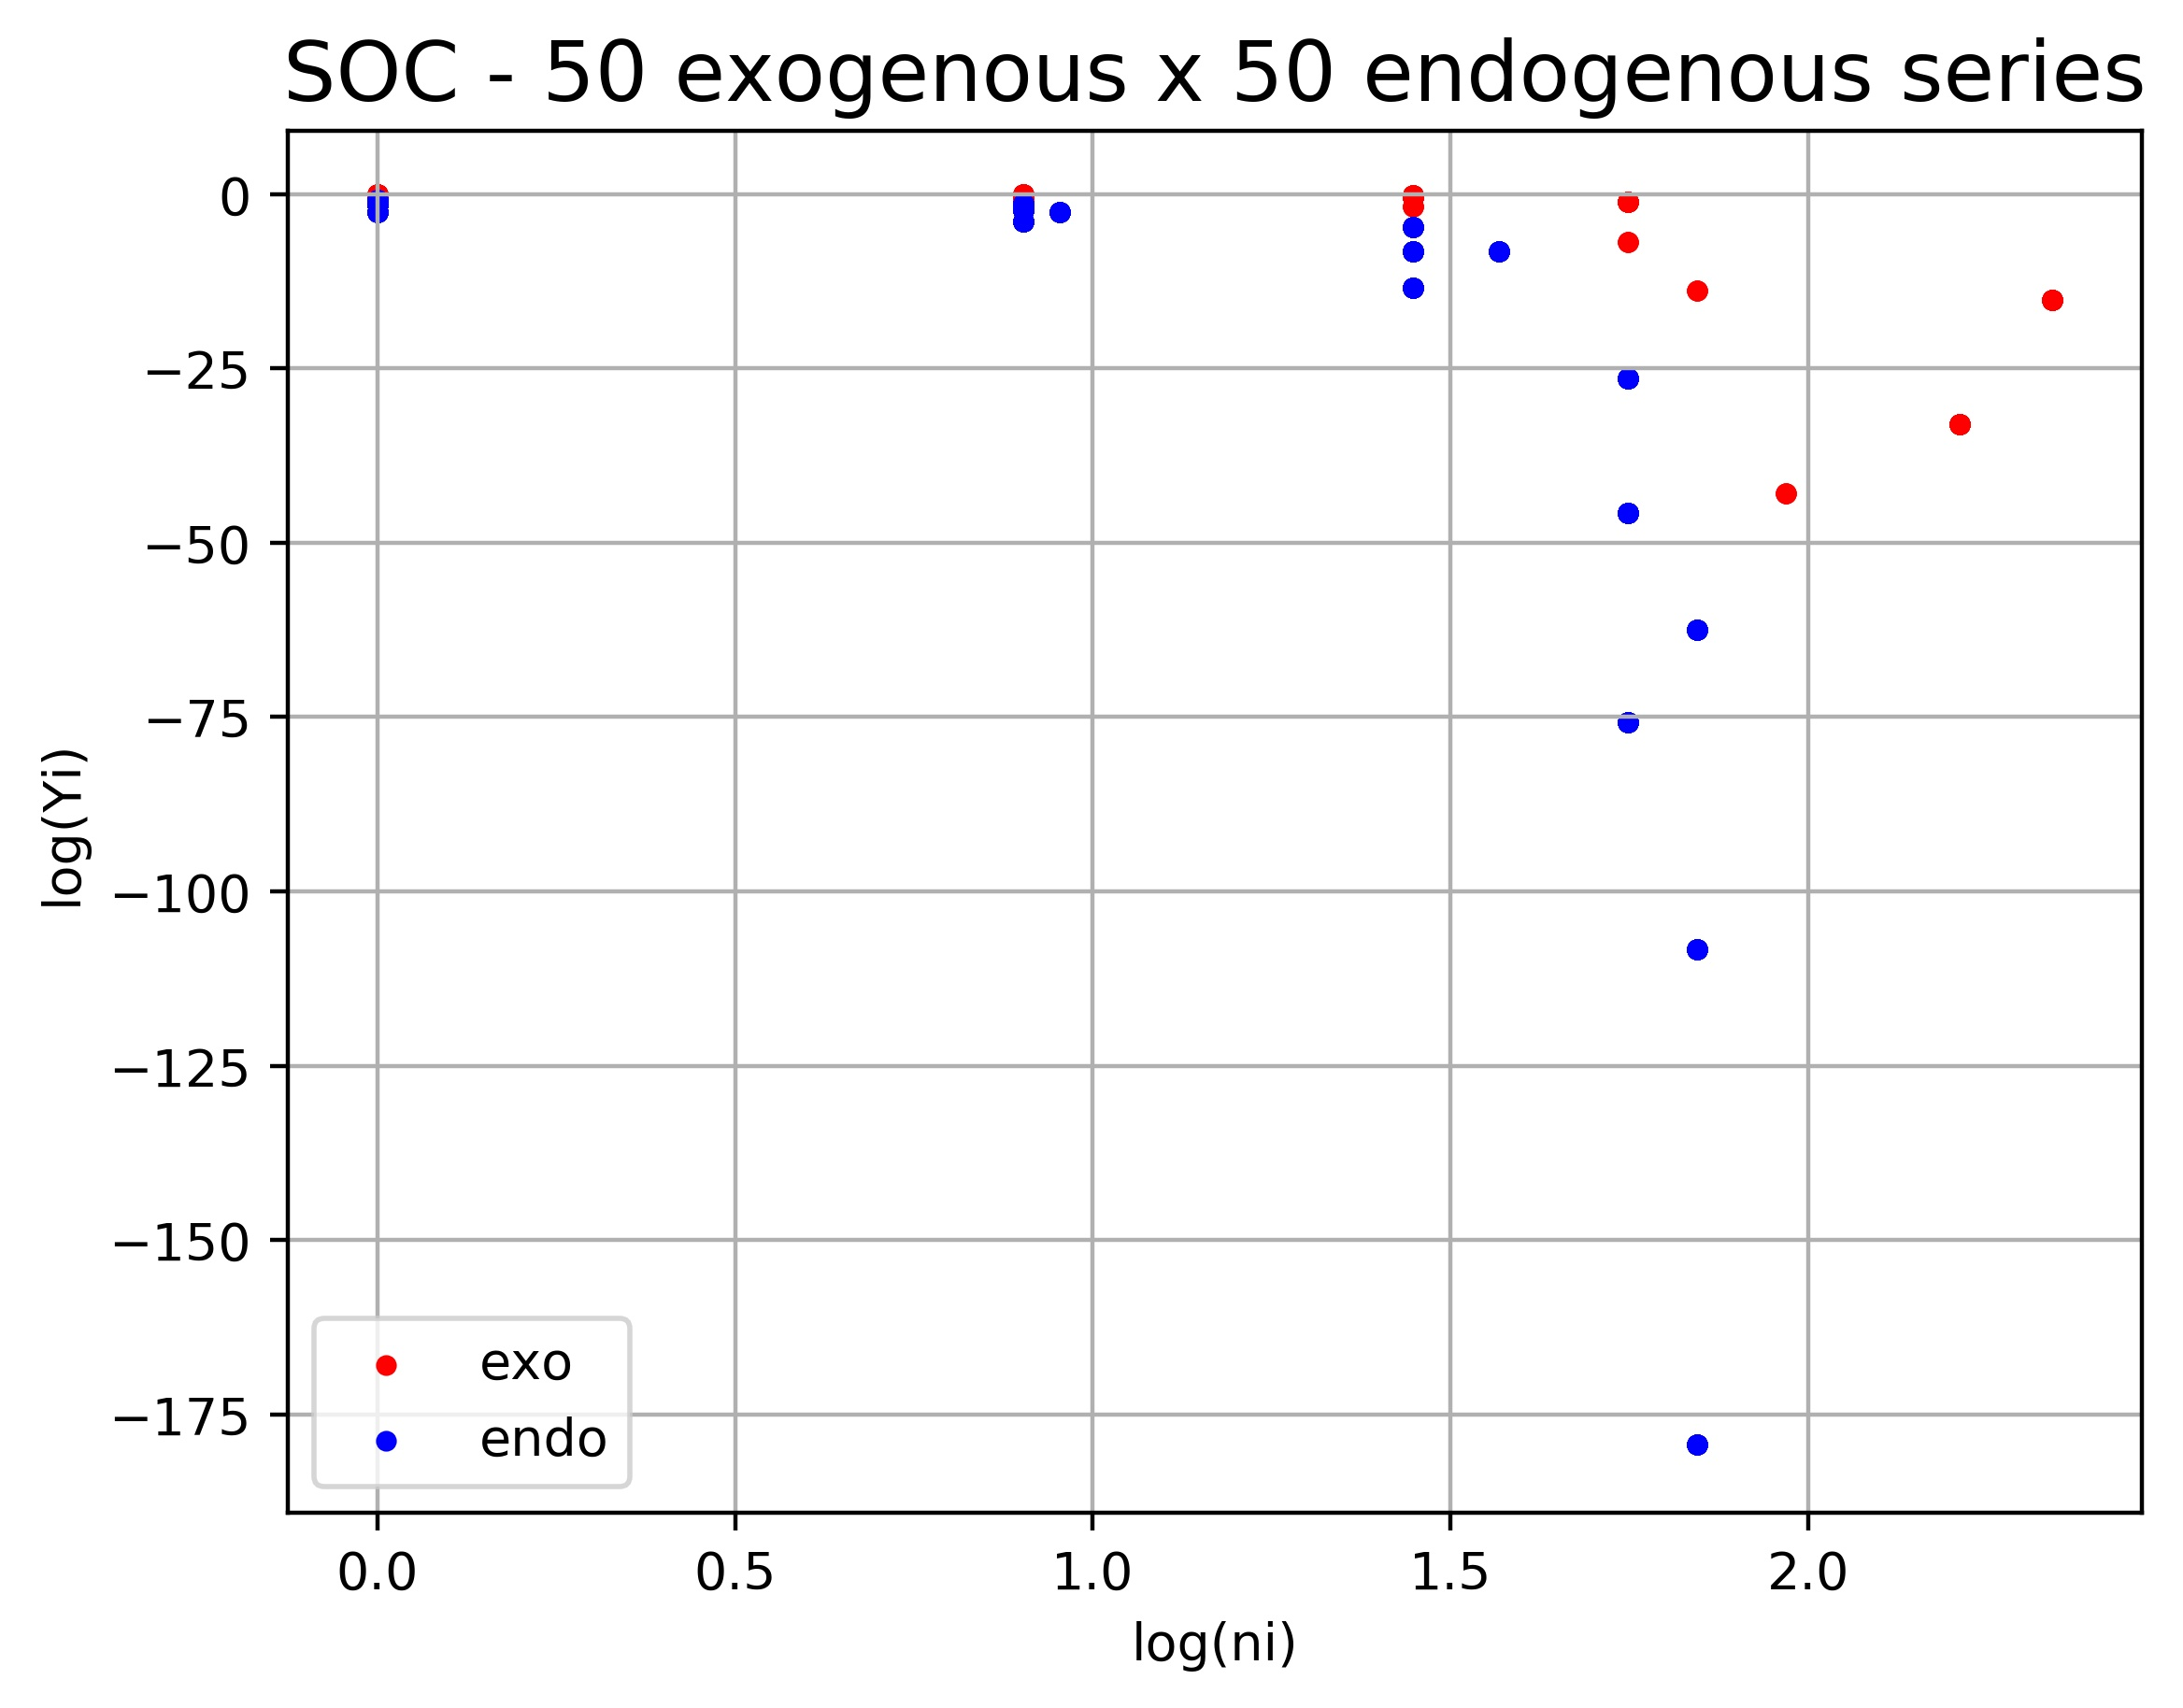
\includegraphics{Figuras/ex9/9_1/Exercicio9_1_exoXendo_SOC.jpg}}		
	\end{center}
	\vspace{-2mm}	% acrescentar o espaçamento vertical apropriado entre a borda inferior da figura e a legenda ou a fonte quando não há legenda (o valor pode ser negativo para subir)
	\legenda{Figura 9.1.1: Plots de Self Organized Criticality para 50 sinais endógenos (em azul) e 50 sinais exógenos (em vermelho). Observa-se que as séries endógenas apresentam perfil de Self Organized Criticality, enquanto as exógenas não.}	% legenda - para deixar sem legenda usar comando \legenda{} (nunca deve-se comentar o comando \legenda)
	\label{ex9_fig1}
	%\FONTE{}	% fonte consultada (elemento obrigatório, mesmo que seja produção do próprio autor)
\end{figure}

\clearpage
\subsection*{9.2}
\addcontentsline{toc}{section}{\protect\numberline{} 9.2}%

Os plots resultantes da análise de todos os países da série \textit{ST-OWS\_NDC\_Covid19} se encontram na pasta \textbf{paises} (dentro da pasta referente a este exercício). A seguir é apresentado o plot do resultado para todos os países da série juntos. O espalhamento de pontos na parte superior do gráfico pode ser interpretado como a presença de diferentes pontos de relaxação para a série, bem como diferentes leis de potência. Além disso, a parte inferior apresenta uma cauda, evidenciando um comportamento de relaxação em um ponto crítico apenas. Ou seja, a menos dos pontos na parte superior do gráfico, há uma assinatura única mais proeminente que pode caracterizar Self Ooganized Criticality.
%Individualmente, os plots de cada país possuem um tamanho pequeno e portanto não são ideais para a análise, mas são importantes pois explicam a distribuição dos pontos na parte superior do plot da Figura 9.2.1. 

\begin{figure}[ht!]
	%\caption{Série e histogramas.}
	\vspace{0mm}	% acrescentar o espaçamento vertical apropriado entre o título e a borda superior da figura
	\begin{center}
		\resizebox{15cm}{!}{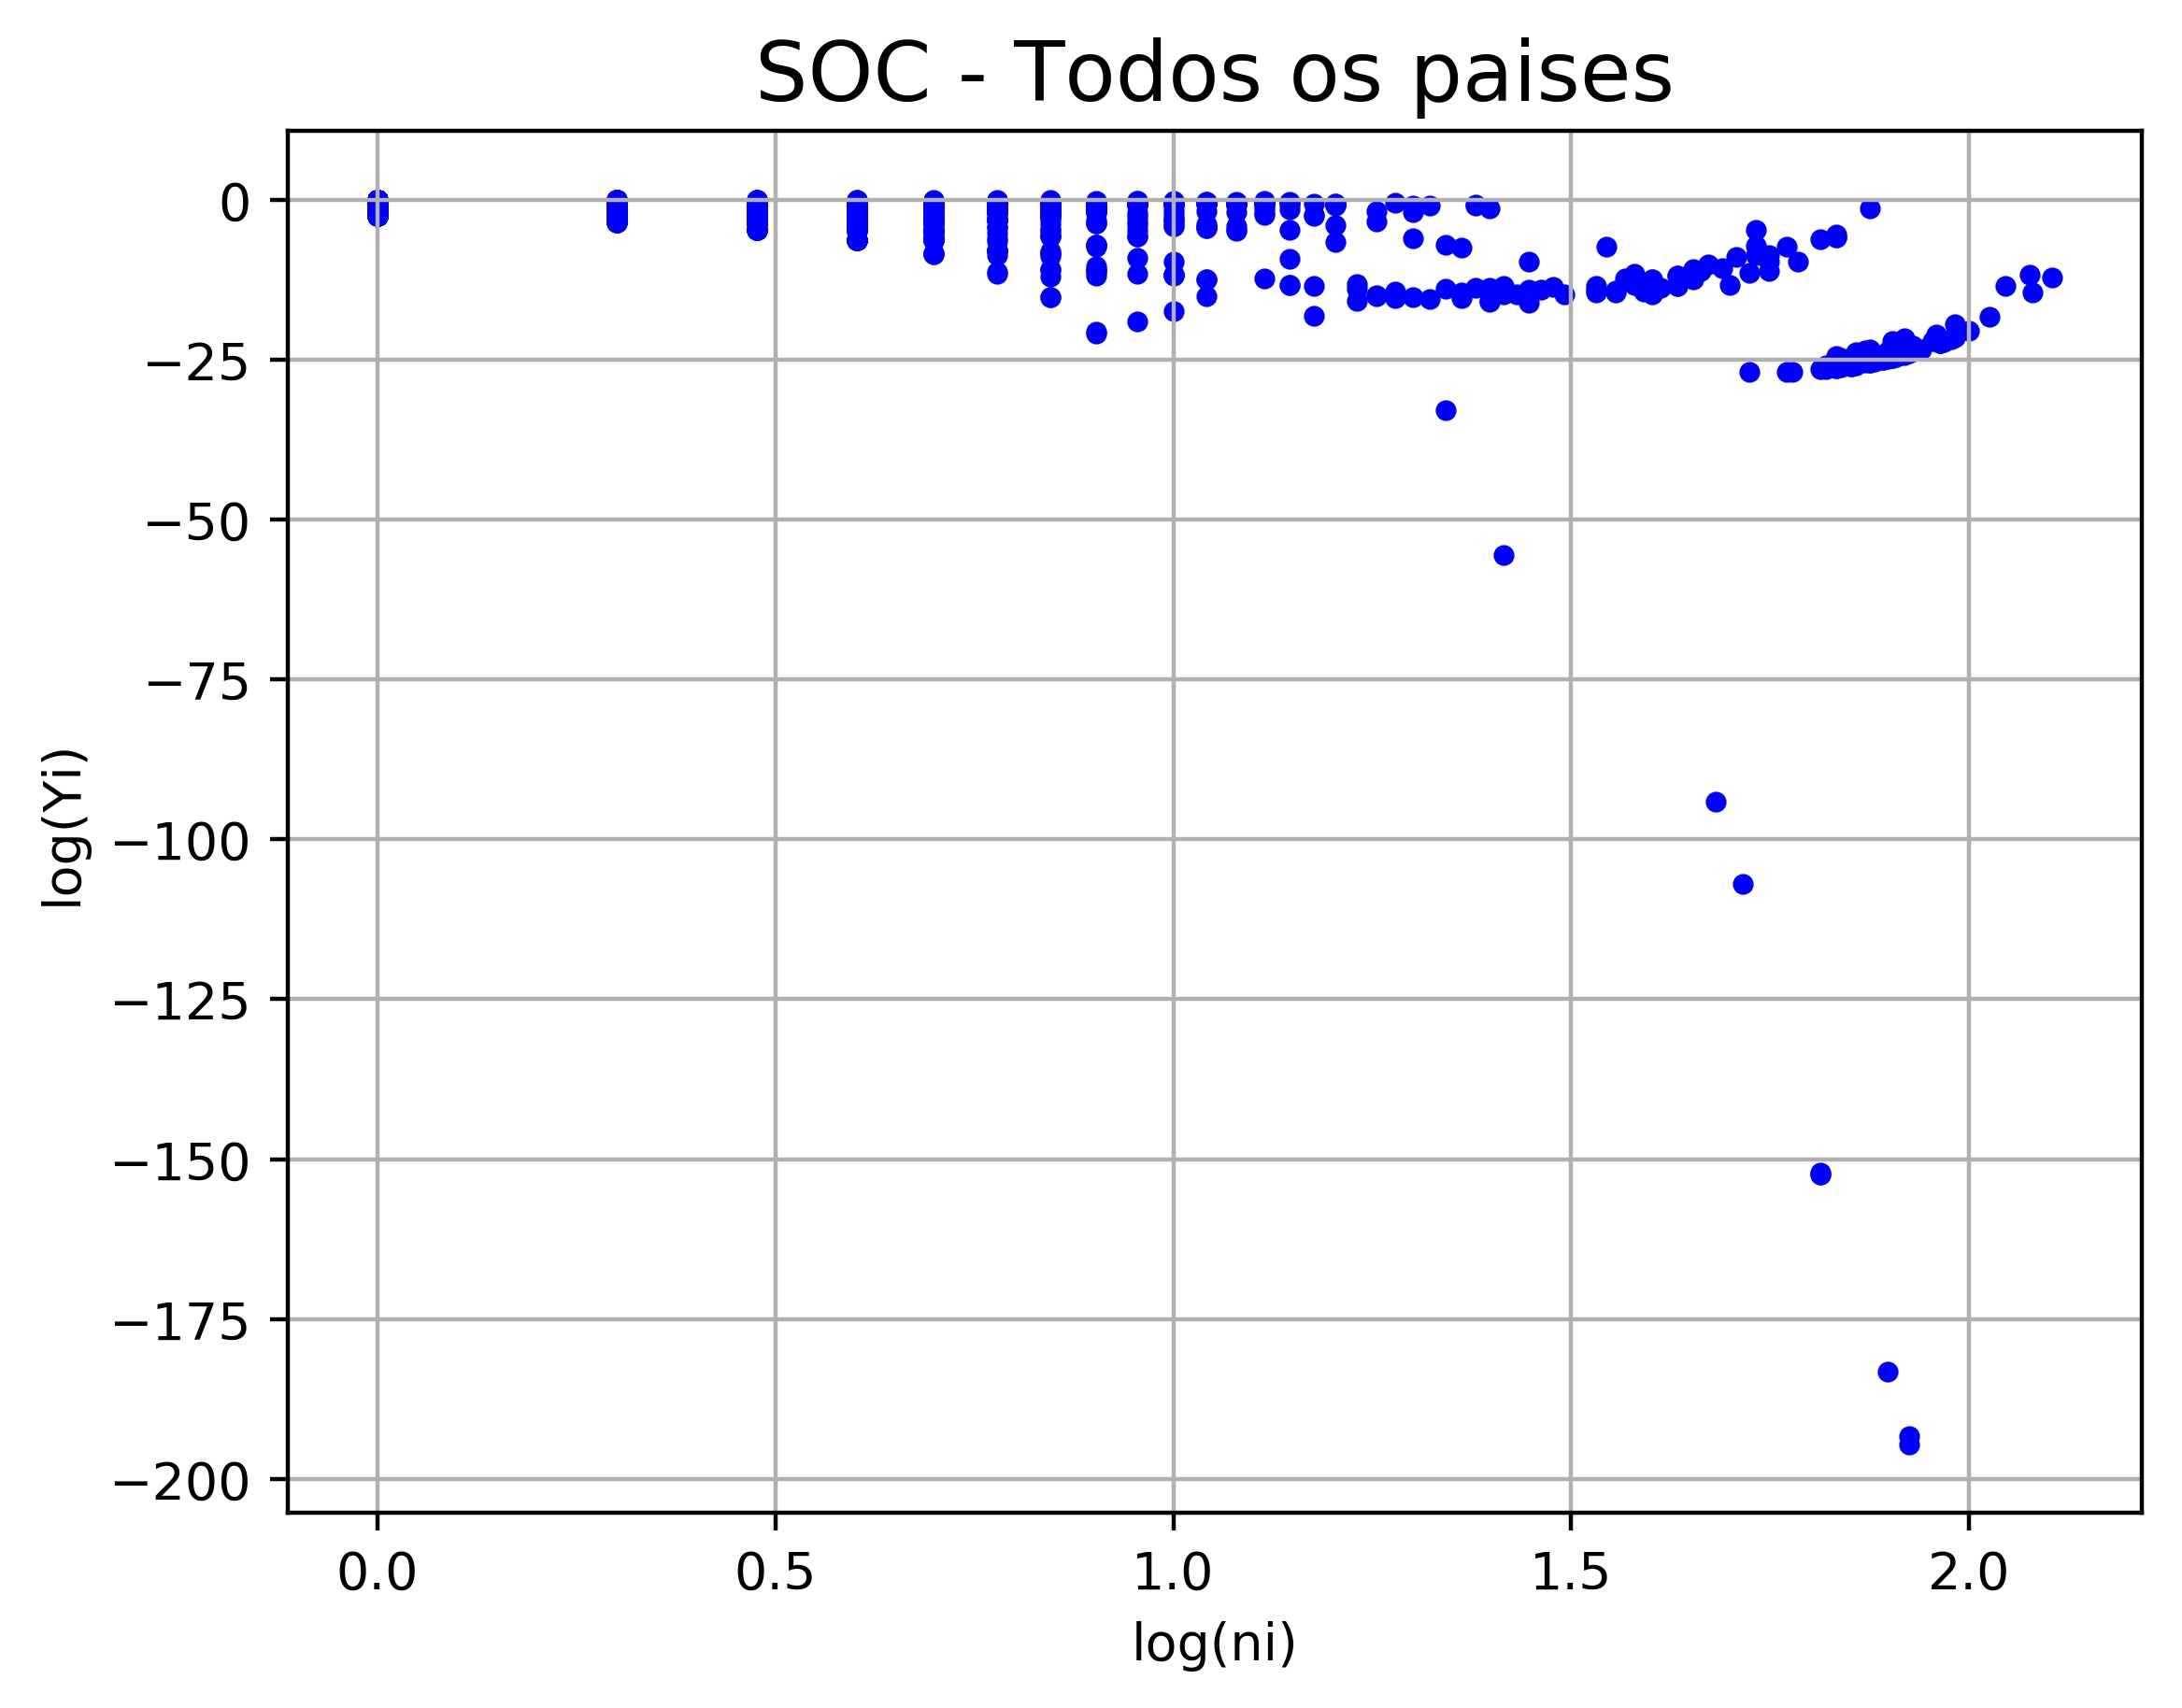
\includegraphics{Figuras/ex9/9_2/Exercicio9_2_todos_os_paises.jpg}}		
	\end{center}
	\vspace{-2mm}	% acrescentar o espaçamento vertical apropriado entre a borda inferior da figura e a legenda ou a fonte quando não há legenda (o valor pode ser negativo para subir)
	\legenda{Figura 9.2.1: Plot de todos os países usando o algoritmo SOC.py.}	% legenda - para deixar sem legenda usar comando \legenda{} (nunca deve-se comentar o comando \legenda)
	\label{ex9_fig1}
	%\FONTE{}	% fonte consultada (elemento obrigatório, mesmo que seja produção do próprio autor)
\end{figure}

%\begin{figure}[ht!]
	%\caption{Série e histogramas.}
%	\vspace{0mm}	% acrescentar o espaçamento vertical apropriado entre o título e a borda superior da figura
%	\begin{center}
%		\resizebox{12cm}{!}{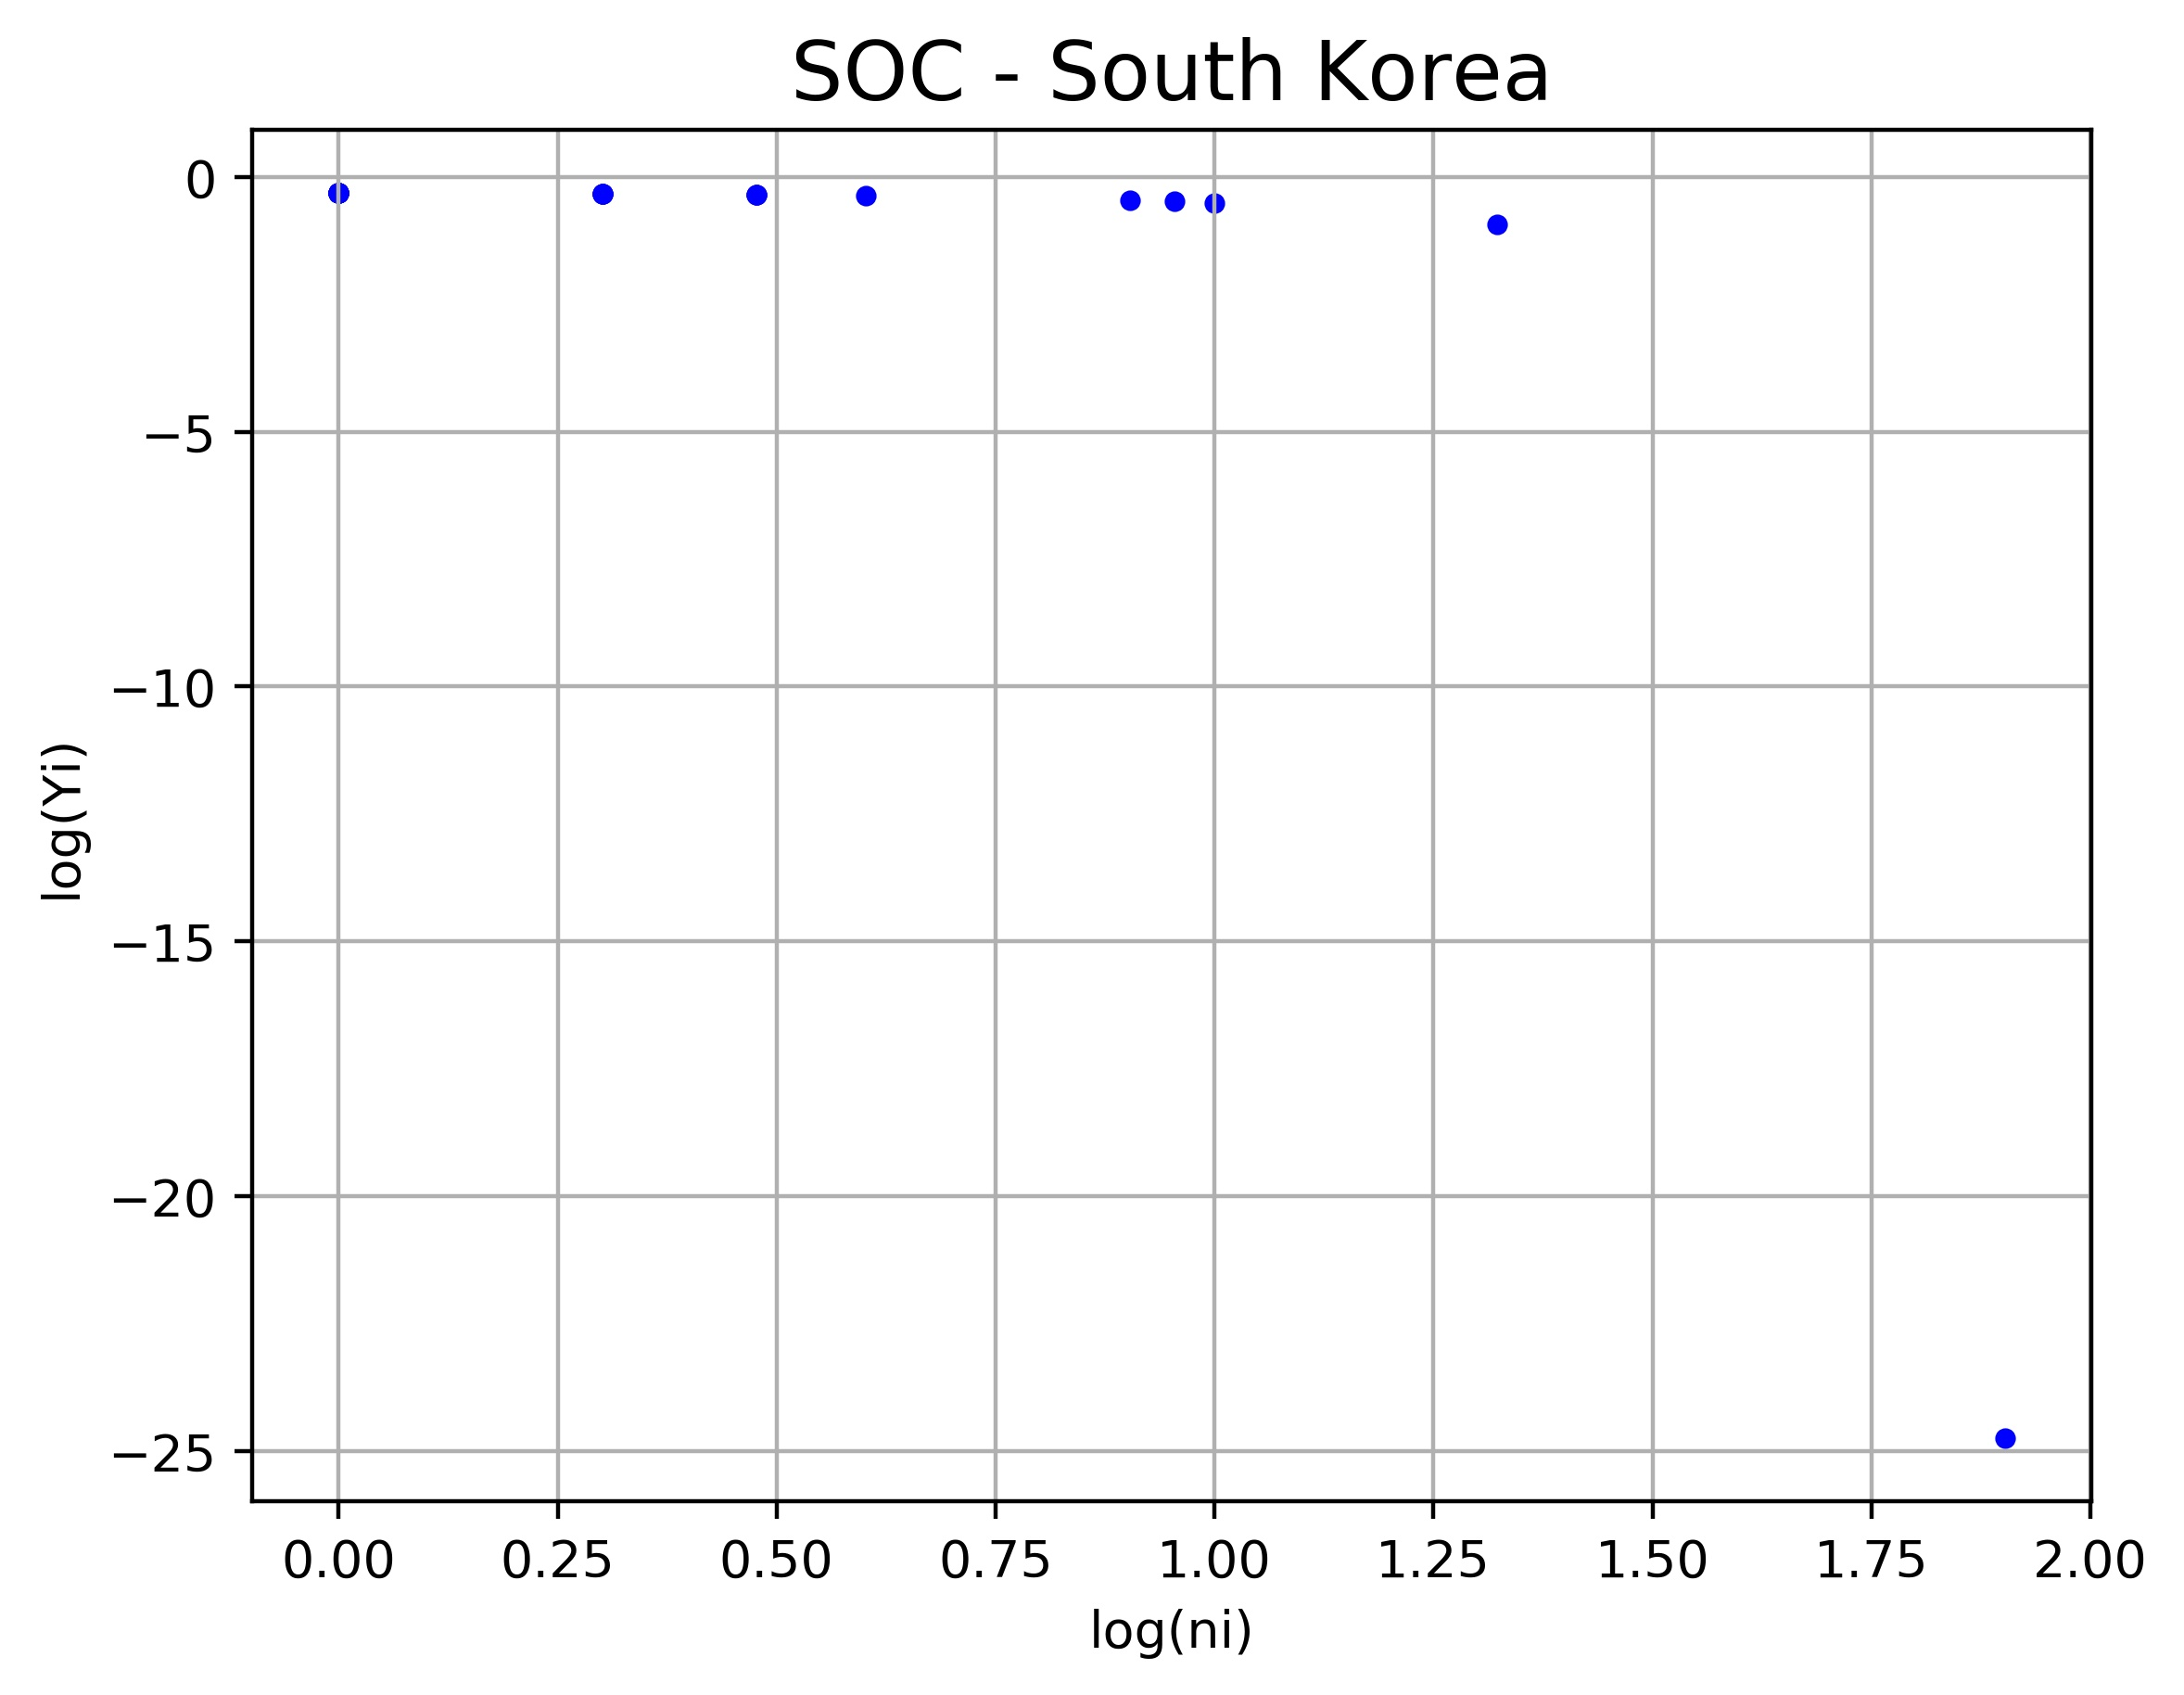
\includegraphics{Figuras/ex9/9_2/Exercicio9_2_South Korea.jpg}}		
%	\end{center}
%	\vspace{-2mm}	% acrescentar o espaçamento vertical apropriado entre a borda inferior da figura e a legenda ou a fonte quando não há legenda (o valor pode ser negativo para subir)
%	\legenda{Figura 9.2.2: Plot da série de novos dados diários da Covid19 para a Coréia do Sul usando o algoritmo SOC.py.}	% legenda - para deixar sem legenda usar comando \legenda{} (nunca deve-se comentar o comando \legenda)
%	\label{ex9_fig1}
	%\FONTE{}	% fonte consultada (elemento obrigatório, mesmo que seja produção do próprio autor)
%\end{figure}

%\begin{figure}[ht!]
	%\caption{Série e histogramas.}
%	\vspace{0mm}	% acrescentar o espaçamento vertical apropriado entre o título e a borda superior da figura
%	\begin{center}
%		\resizebox{12cm}{!}{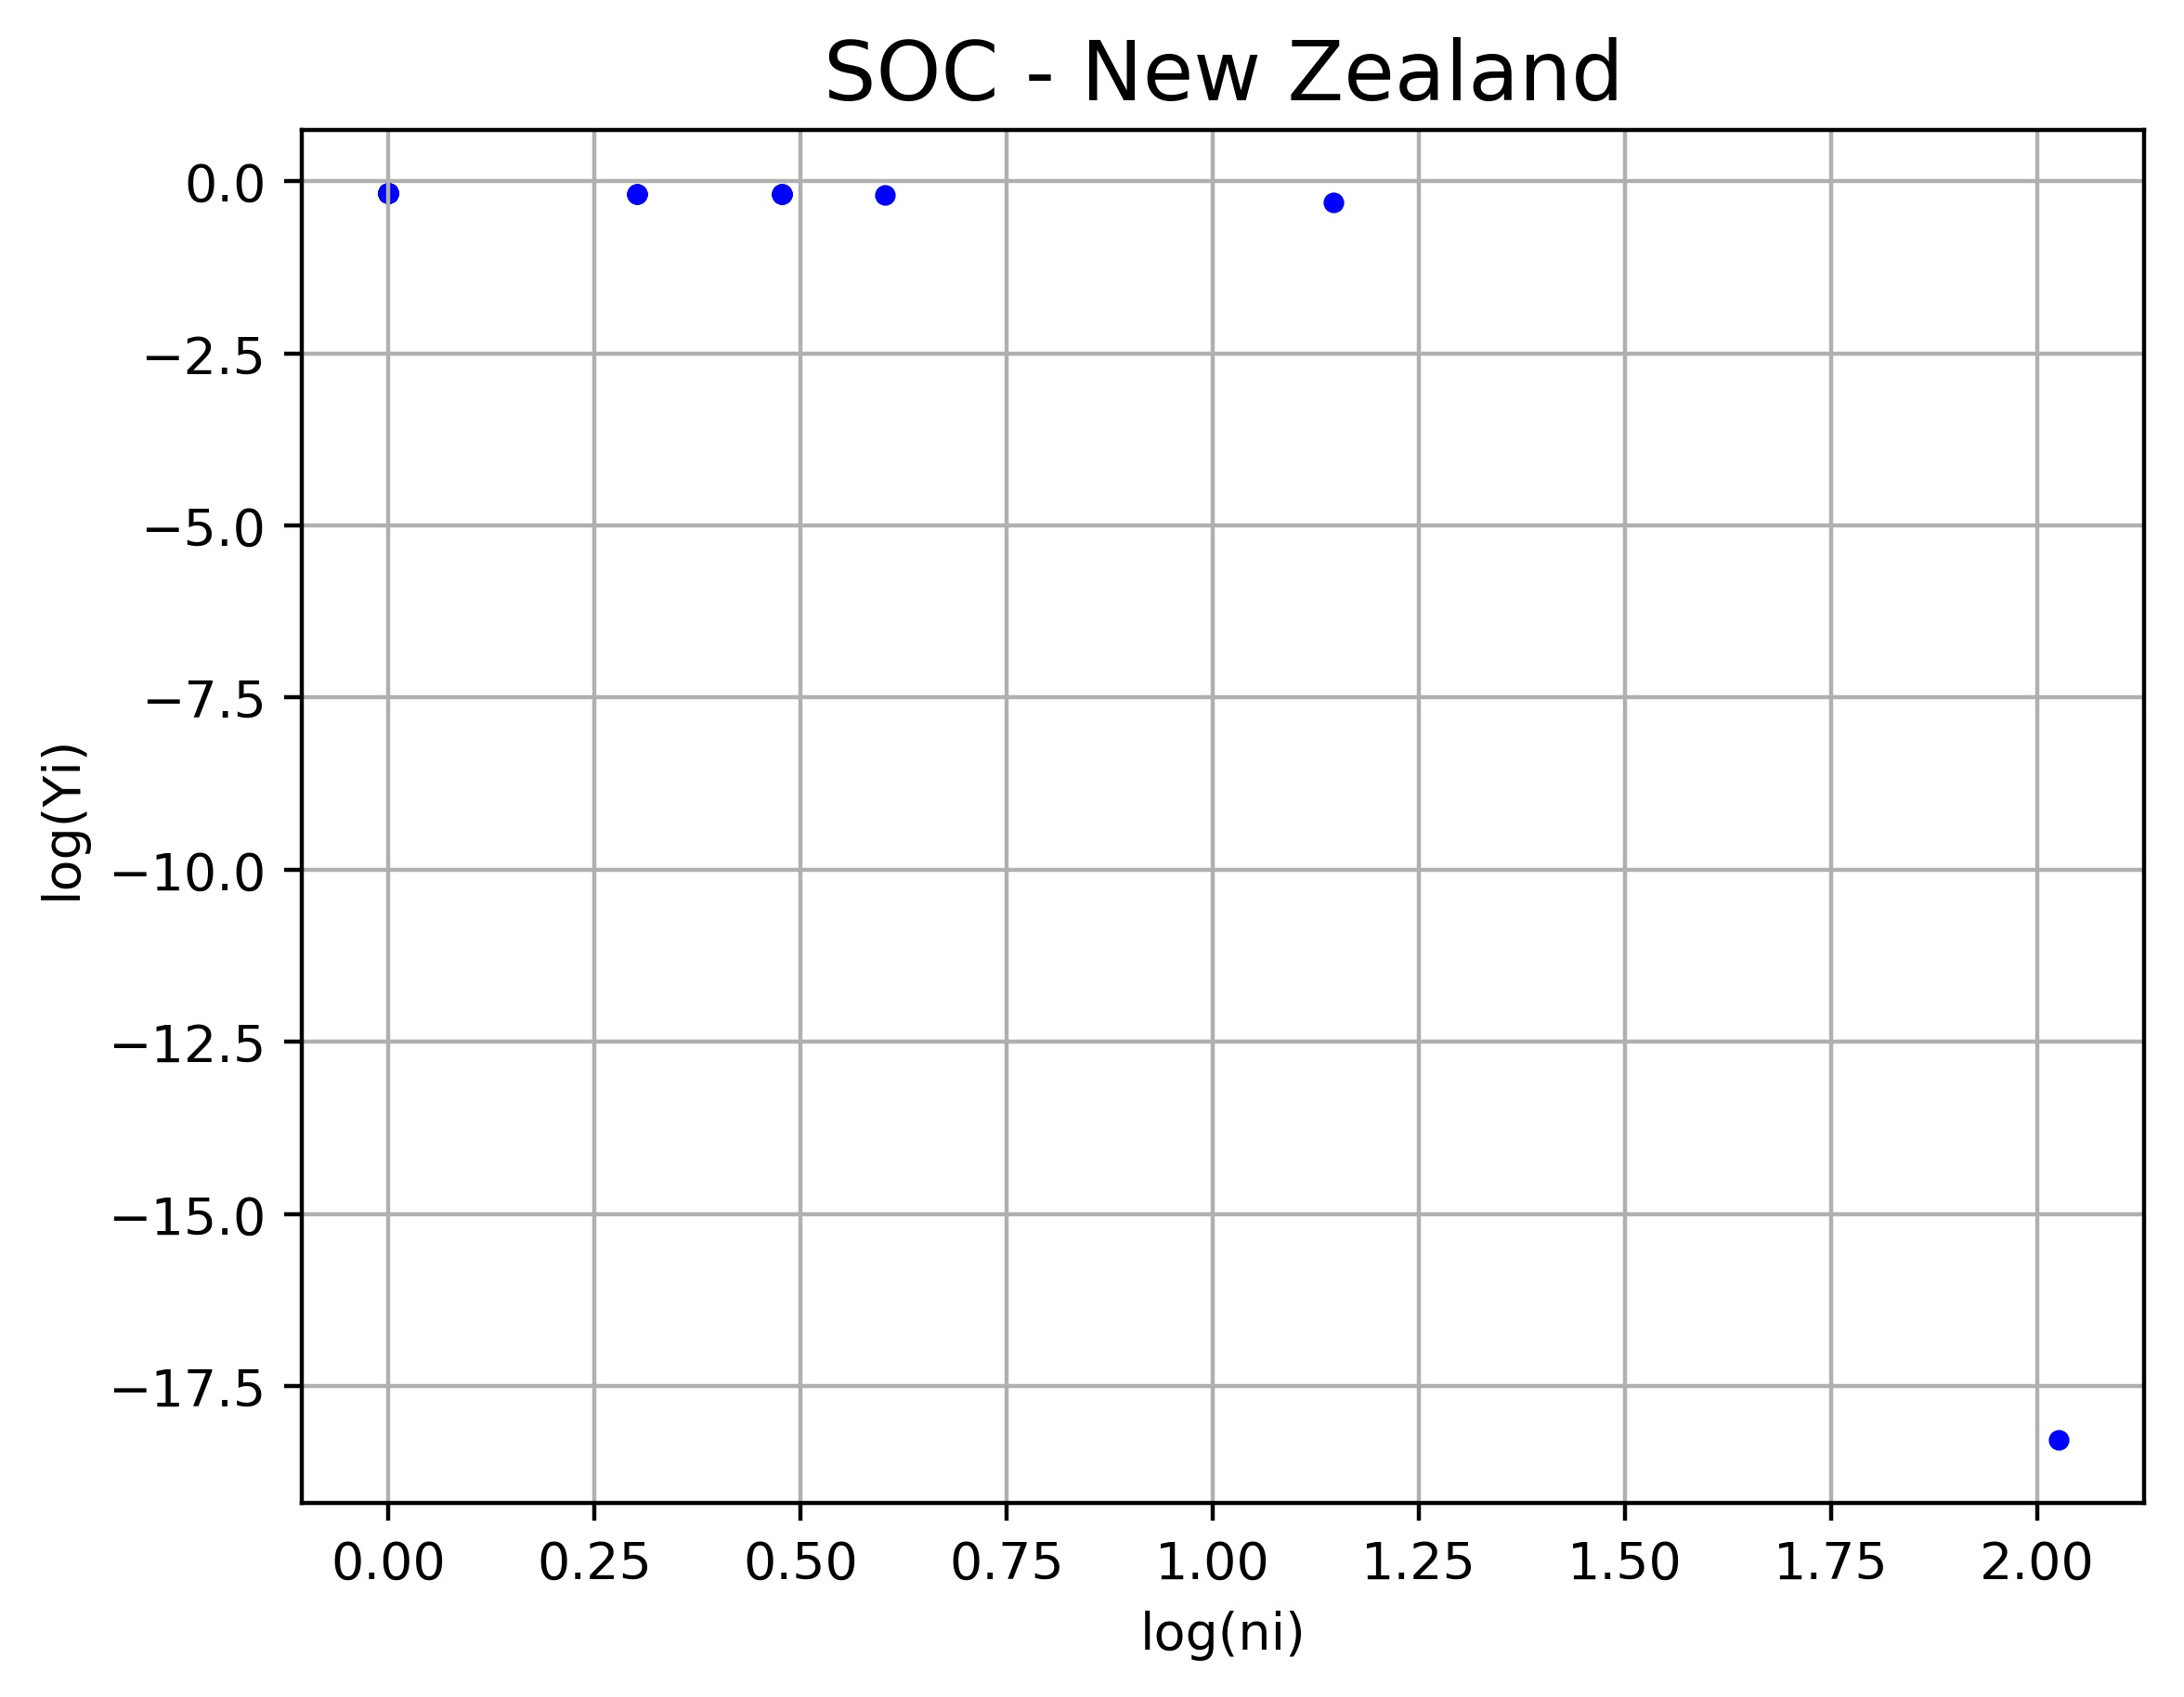
\includegraphics{Figuras/ex9/9_2/Exercicio9_2_New Zealand.jpg}}		
%	\end{center}
%	\vspace{-2mm}	% acrescentar o espaçamento vertical apropriado entre a borda inferior da figura e a legenda ou a fonte quando não há legenda (o valor pode ser negativo para subir)
%	\legenda{Figura 9.2.3: Plot da série de novos dados diários da Covid19 para a Nova Zelândia usando o algoritmo SOC.py.}	% legenda - para deixar sem legenda usar comando \legenda{} (nunca deve-se comentar o comando \legenda)
%	\label{ex9_fig1}
	%\FONTE{}	% fonte consultada (elemento obrigatório, mesmo que seja produção do próprio autor)
%\end{figure}

%\begin{figure}[ht!]
	%\caption{Série e histogramas.}
%	\vspace{0mm}	% acrescentar o espaçamento vertical apropriado entre o título e a borda superior da figura
%	\begin{center}
%		\resizebox{12cm}{!}{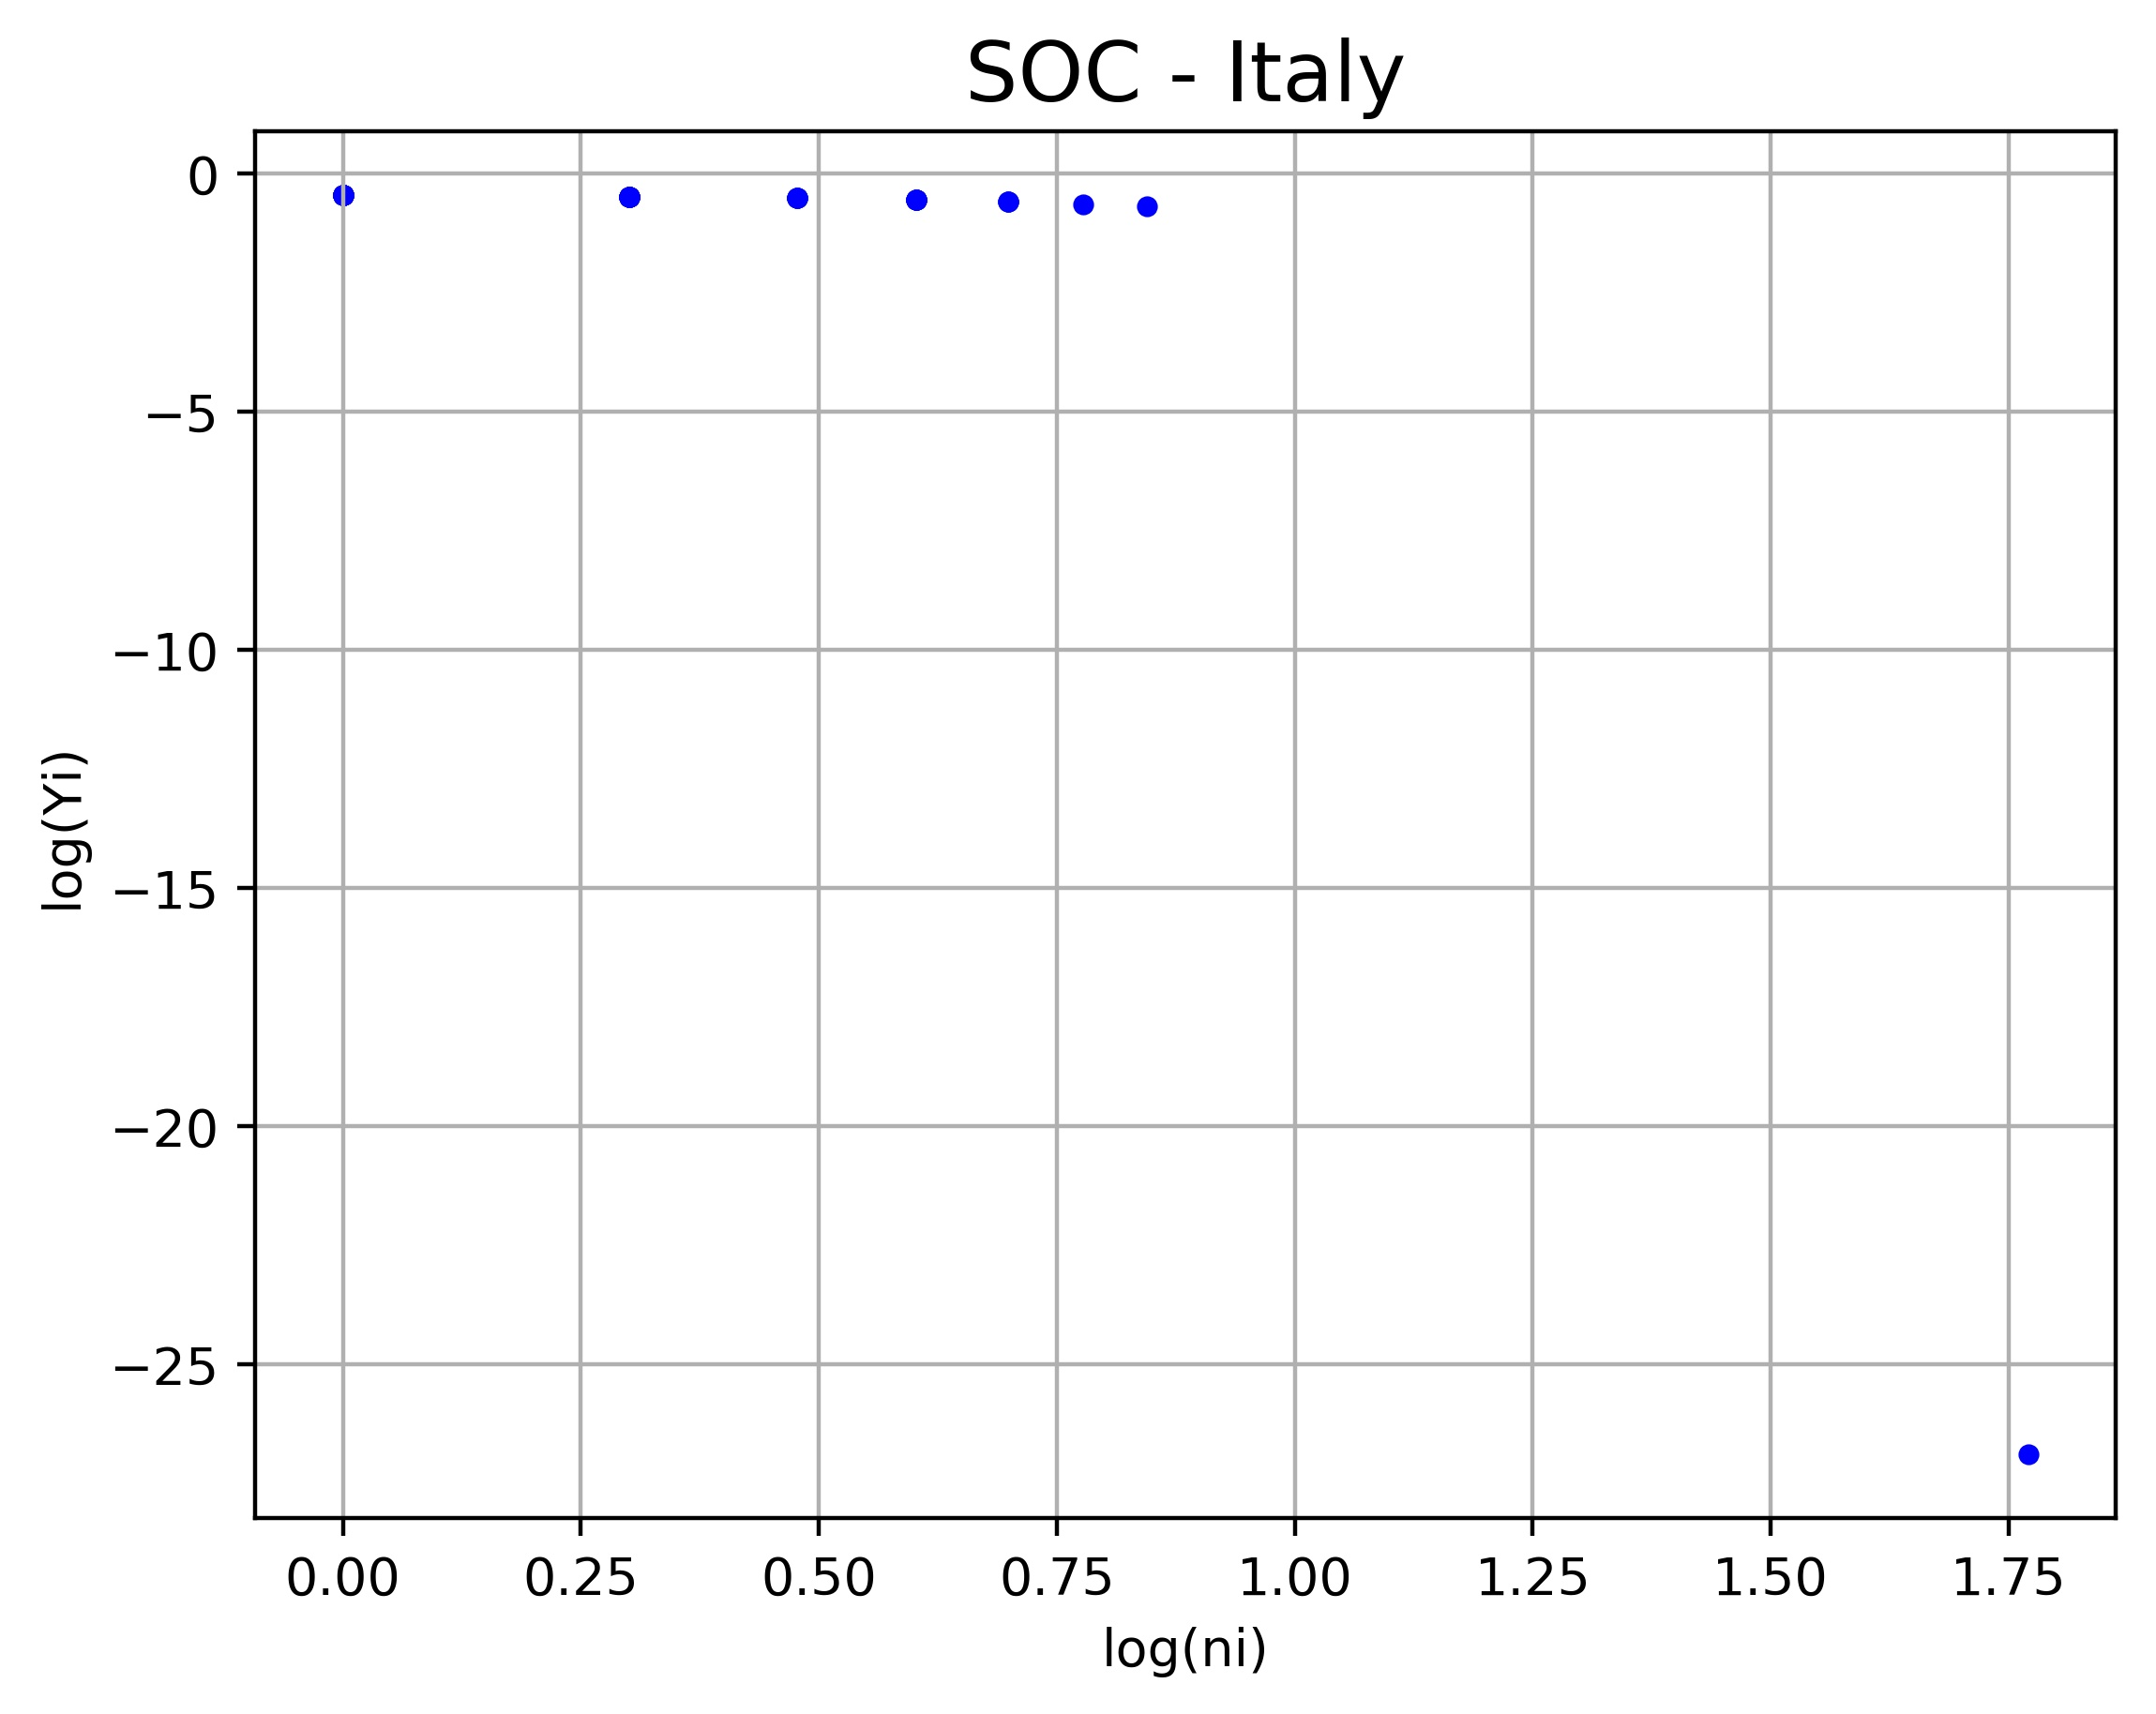
\includegraphics{Figuras/ex9/9_2/Exercicio9_2_Italy.jpg}}		
%	\end{center}
%	\vspace{-2mm}	% acrescentar o espaçamento vertical apropriado entre a borda inferior da figura e a legenda ou a fonte quando não há legenda (o valor pode ser negativo para subir)
%	\legenda{Figura 9.2.4: Plot da série de novos dados diários da Covid19 para a Itália usando o algoritmo SOC.py.}	% legenda - para deixar sem legenda usar comando \legenda{} (nunca deve-se comentar o comando \legenda)
%	\label{ex9_fig1}
	%\FONTE{}	% fonte consultada (elemento obrigatório, mesmo que seja produção do próprio autor)
%\end{figure}

%\begin{figure}[ht!]
%	%\caption{Série e histogramas.}
%	\vspace{0mm}	% acrescentar o espaçamento vertical apropriado entre o título e a borda superior da figura
%	\begin{center}
%		\resizebox{12cm}{!}{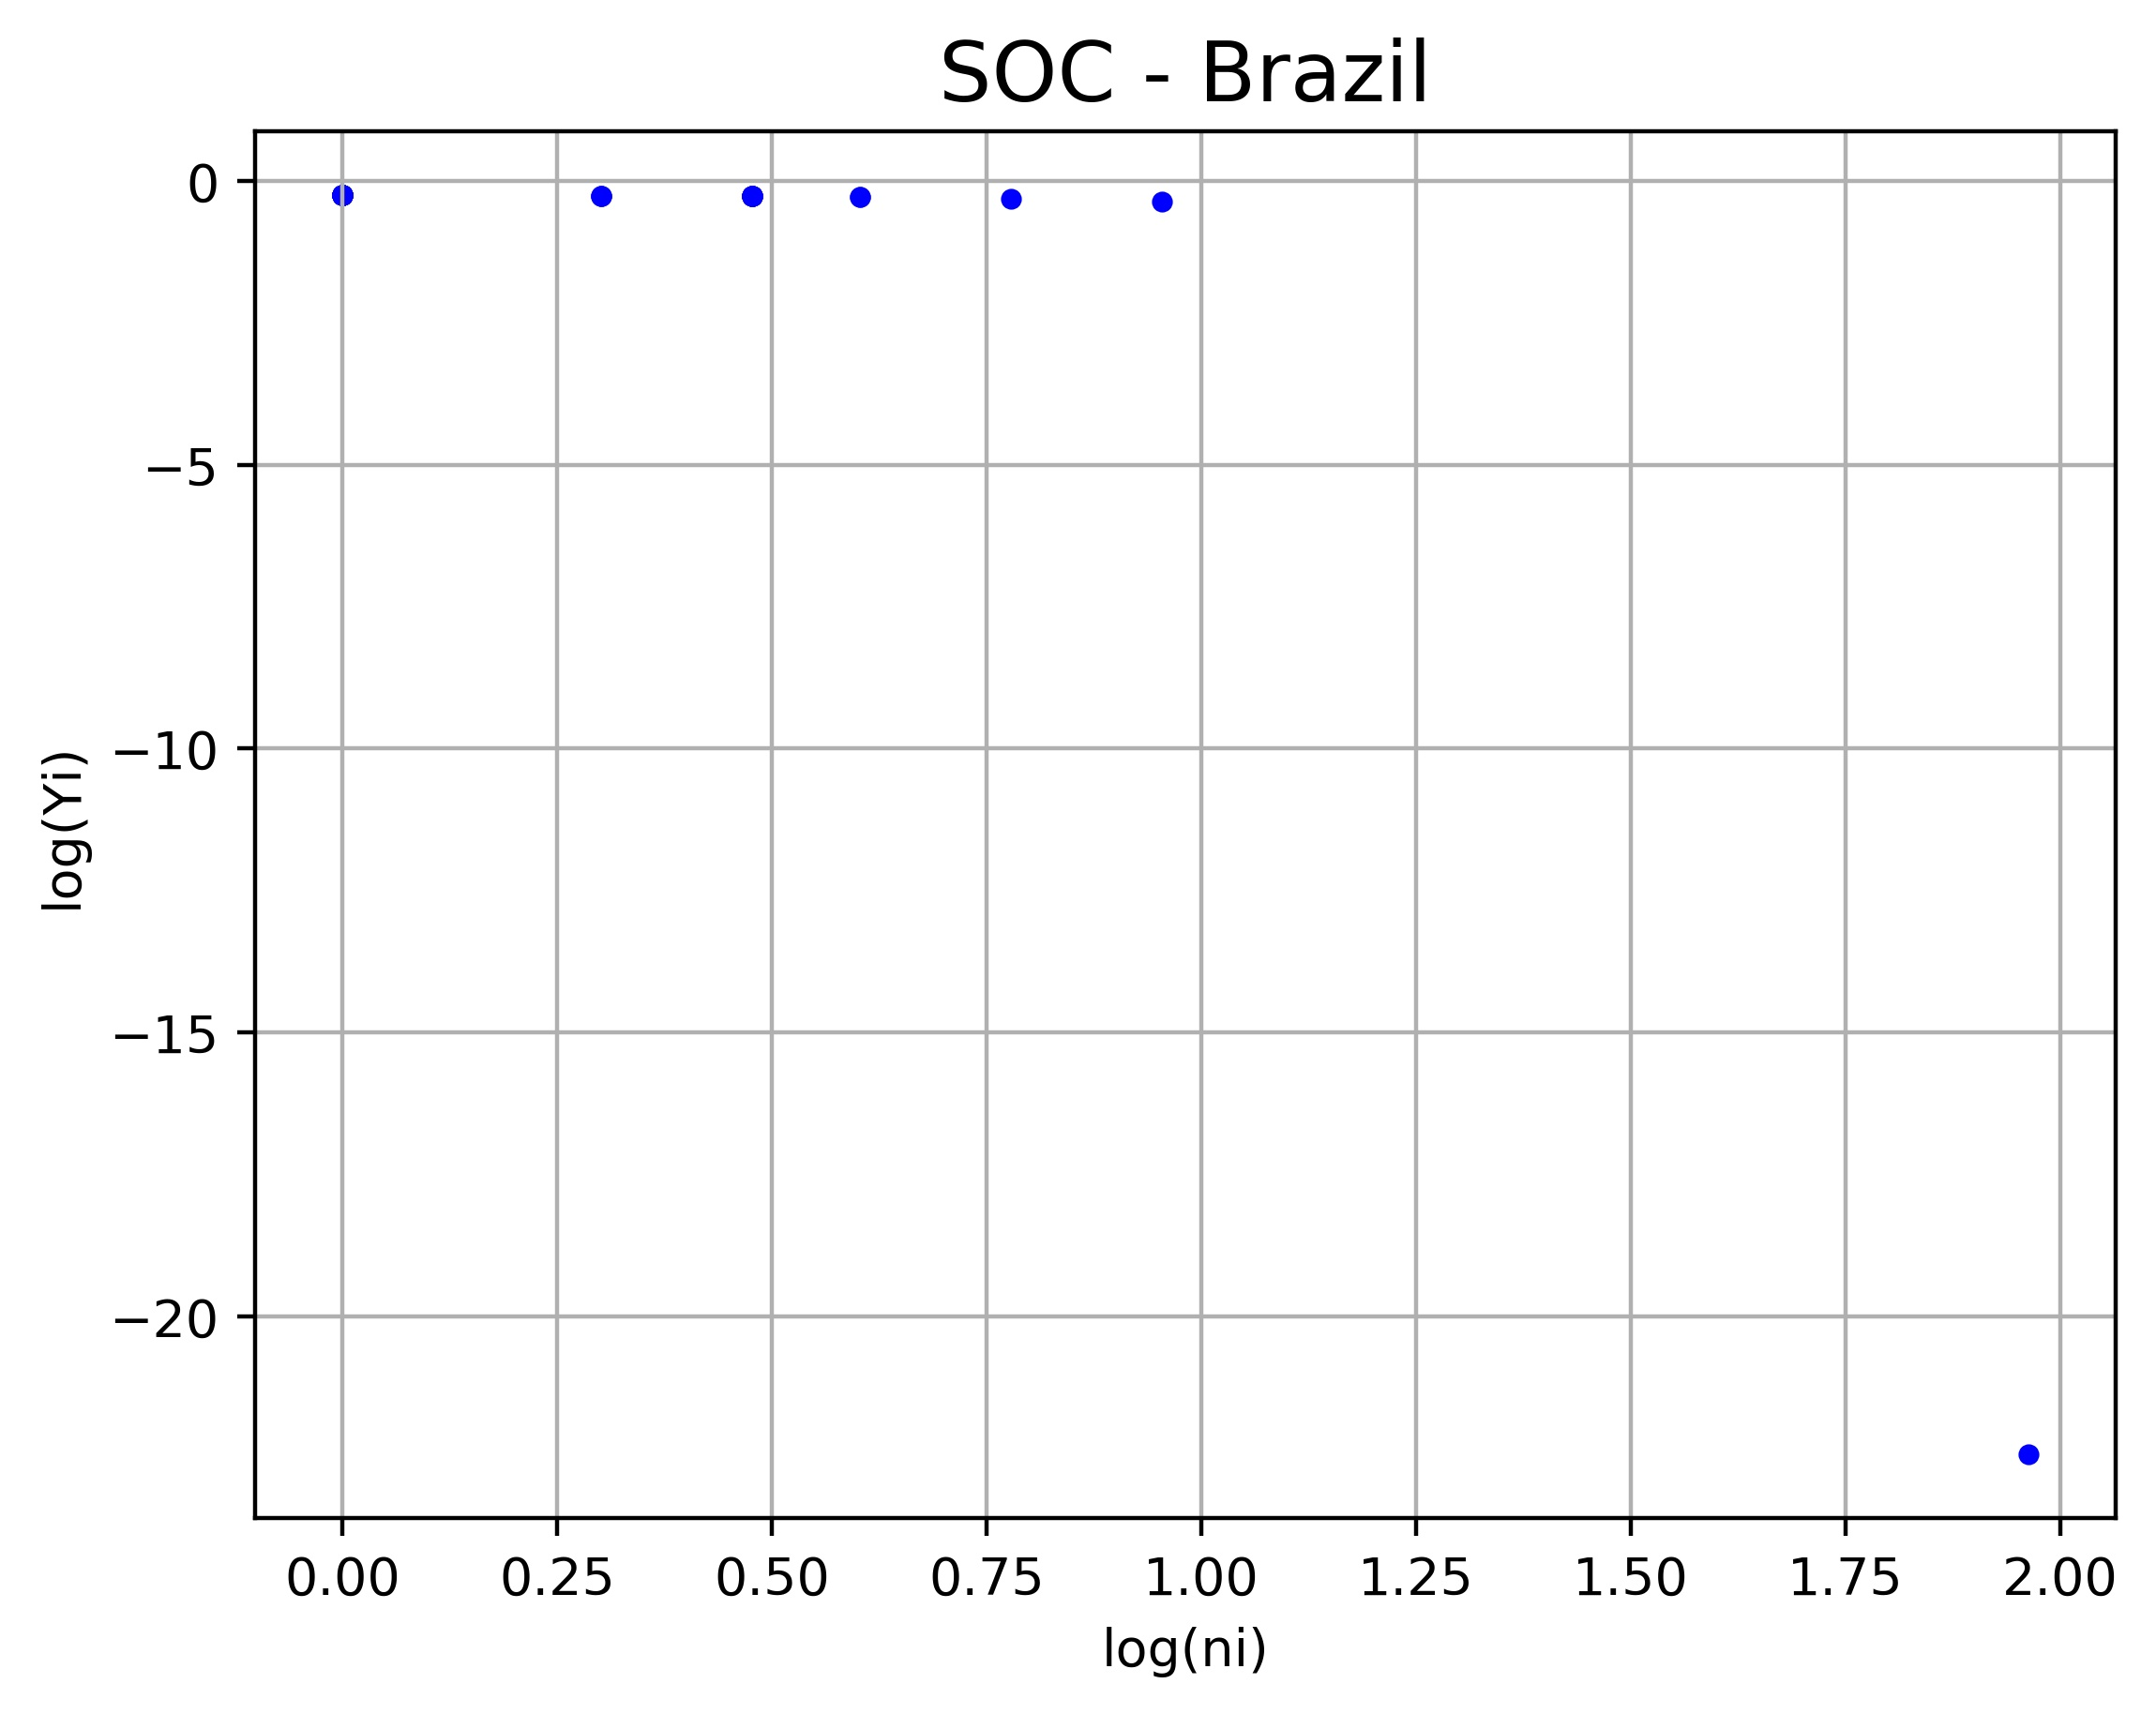
\includegraphics{Figuras/ex9/9_2/Exercicio9_2_Brazil.jpg}}		
%	\end{center}
%	\vspace{-2mm}	% acrescentar o espaçamento vertical apropriado entre a borda inferior da figura e a legenda ou a fonte quando não há legenda (o valor pode ser negativo para subir)
%	\legenda{Figura 9.2.5: Plot da série de novos dados diários da Covid19 para o Brasil usando o algoritmo SOC.py.}	% legenda - para deixar sem legenda usar comando \legenda{} (nunca deve-se comentar o comando \legenda)
%	\label{ex9_fig1}
	%\FONTE{}	% fonte consultada (elemento obrigatório, mesmo que seja produção do próprio autor)
%\end{figure}



